\documentclass[10pt, twocolumn]{article}
\usepackage[margin=1in]{geometry}
\usepackage{lmodern}% http://ctan.org/pkg/lm
\usepackage{authblk} % adds affiliations

\usepackage[utf8x]{inputenc}
\usepackage{nameref}
\usepackage[switch]{lineno}
\usepackage{amsmath}
\usepackage{booktabs}
\usepackage[numbers,super]{natbib}
\usepackage{changepage}

% adjust caption style
\usepackage[aboveskip=1pt,labelfont=bf,
            labelsep=period,singlelinecheck=off]{caption}

% remove brackets from references
\makeatletter
\renewcommand{\@biblabel}[1]{\quad#1.}
\makeatother

\usepackage[colorinlistoftodos]{todonotes}

% headrule, footrule and page numbers
\usepackage{lastpage,fancyhdr,graphicx}
\usepackage{epstopdf}
\pagestyle{myheadings}
\pagestyle{fancy}
\fancyhf{}
\rfoot{\thepage/\pageref{LastPage}}
\renewcommand{\footrule}{\hrule height 2pt \vspace{2mm}}

% use \textcolor{color}{text} for colored text (e.g. highlight to-do areas)
\usepackage{color}

\definecolor{Gray}{gray}{.25}

\usepackage{graphicx}

% use if you want to put caption to the side of the figure
\usepackage{sidecap}

\usepackage{xcolor}
\usepackage[colorlinks = true,
            linkcolor = blue,
            urlcolor  = blue,
            citecolor = blue,
            anchorcolor = blue]{hyperref}

% ####################################################
% ####################################################
\usepackage[colorinlistoftodos]{todonotes}
% ####################################################
% ####################################################

% use for have text wrap around figures
\usepackage{wrapfig}
\usepackage[pscoord]{eso-pic}
\usepackage[fulladjust]{marginnote}
\reversemarginpar{}

\usepackage{gensymb}
\usepackage{siunitx}

% make a box for author summary
\usepackage[framemethod=TikZ]{mdframed}
%% define the style
\newcommand{\mybox}[2]{%
         \begin{center}%
            \begin{tikzpicture}%
                \node[rectangle, draw=#1, top color=#1!10, bottom color=#1!10,
                      rounded corners=5pt, inner xsep=5pt, inner ysep=6pt,
                      outer ysep=10pt]{
                        \begin{minipage}{1\textwidth}#2\end{minipage}};%
            \end{tikzpicture}%
         \end{center}%
}

% new commands
% q value
\newcommand{\qval}[1]{$q<10^{-#1}$}

% species names
\newcommand{\cel}{\emph{C.~elegans}}
\newcommand{\dicty}{\emph{D.~discoideum}}
\newcommand{\ecol}{\emph{E.~coli}}
\newcommand{\gf}{gain-of-function allele}
\newcommand{\lf}{loss-of-function allele}
\newcommand{\strong}{strong loss-of-function allele}
\newcommand{\weak}{weak loss-of-function allele}

% gene names
% \newcommand{\gene}[1]{\emph{#1}} # for MS word typesetting
\newcommand{\gene}[1]{\mbox{\emph{#1}}}
\newcommand{\genotype}[1]{\mbox{\emph{#1}}}
\newcommand{\protein}[1]{\mbox{\uppercase{#1}}}
\newcommand{\ras}{\gene{let-60} (\emph{ras})}
\newcommand{\rasp}{\protein{let-60}}
\newcommand{\dpy}{\gene{mdt-12}}
\newcommand{\letgfn}{3,021}
\newcommand{\letlfn}{857}
\newcommand{\letgf}{\gene{let-60(gf)}}
\newcommand{\letlf}{\gene{let-60(lf)}}
\newcommand{\strongn}{2,863}
\newcommand{\weakn}{481}
\newcommand{\transn}{2,214}


% more space between rows
\newcommand{\ra}[1]{\renewcommand{\arraystretch}{#1}}

\title{A study of allelic series using transcriptomic phenotypes}

\author[1]{David Angeles-Albores}
\author[1,*]{Paul W. Sternberg}
\affil[1]{Division of Biology and Biological Engineering, Caltech,
Pasadena, CA, 91125, USA}
\affil[*]{Corresponding author. Contact: pws@caltech.edu}
\renewcommand\Affilfont{\itshape\small{}}

% document begins here
\begin{document}
% title

\twocolumn[
  \begin{@twocolumnfalse}
    \maketitle
    % \section*{Abstract}
    \textbf{Expression profiling holds great promise for genetics because of its
    ability to measure thousands of genes quantitatively in parallel. Although
    transcriptomes have recently been used to perform epistasis analyses for
    pathway reconstruction, there has not been a systematic effort to understand
    how expression profiles will vary among various mutants of the same gene.
    Here, we study an allelic series in \cel{} consisting of one wild type and
    two mutant alleles of \dpy{}, a highly pleiotropic gene whose gene product
    is a subunit of Mediator complex, which is essential for transcriptional
    initiation in eukaryotes. We developed a false hit analysis to identify
    which populations of genes commonly differentially expressed with respect to
    the wild type are likely the result of statistical artifact. We concluded
    that expression perturbations caused by these alleles split into four
    distinct modules called phenotypic classes. To understand the dominance
    relationship between the two mutant alleles, we developed a dominance
    analysis for transcriptional data. Dominance analysis of these phenotypic
    classes support a model where \dpy{} has multiple functional units that
    function independently to target the Mediator complex to specific genetic
    loci.
    }
    \vspace{5mm}

    \mybox{red}{
    \section*{Author Summary}
    Expression profiling is a way to quickly and quantitatively measure the expression
    level of every gene in an organism. As a result, these profiles could be used as
    phenotypes with which to perform genetic analyses (i.e., to figure out what genes
    interact with each other) as well as to dissect the molecular properties of each
    gene. Before we can perform these analyses, we have to figure out the rules that
    apply to these measurements. In this paper, we develop new concepts and methods
    with which to study an allelic series. Briefly, allelic series are an important
    aspect of genetics because different alleles encode different versions of a gene.
    By studying these different versions, we can make statements about how function
    is encoded within the sequence of a gene. We apply our methods to the \dpy{}
    gene, which encodes a subunit of the Mediator complex.
    Though we know it is essential for all transcriptional activity in eukaryotes,
    we understand very little about how the Mediator complex functions to generate
    both general and specific phenotypes. The reason for this is the genes that
    encode these subunits are associated with general sickness and multiple
    phenotypes when mutated, which makes them challenging to study genetically.
    We show that transcriptomic phenotypes renders the study of general factors
    such as \dpy{} feasible.
    }
    \vspace{2mm}

    \mybox{blue}{
    \section*{Supplementary Data}
    The website for the Supplementary Data for this project is still under
    construction and will be available shortly. All code, data and figures are
    available upon request.
    }
    \vspace{5mm}

  \end{@twocolumnfalse}
]


\linenumbers{}

\section*{Introduction}
The term `allelic series' refers to the study of alleles with different
phenotypes to understand the molecular properties that this locus controls.
Allelic series are historically important for genetics~\cite{McClintock1944}.
In early pioneering work, McClintock studied a deficiency of the tail end of
chromosome 9 of maize by generating \emph{trans}-heterozygotes with mutants of
various genes that she knew existed near the end of chromosome 9. Her work
allowed her to infer that the deficiency was modular, effectively generating a
double mutant that behaved as a single allele but which could participate
phenotypically in two distinct allelic series. From this study, McClintock
inferred that deletions could span multiple genes, which behaved as independent
modules, and which were identified via complementation assays. This work set the
foundations for later observations in yeast that showed two mutant alleles of
the same genetic unit, when placed in \emph{trans} to each other, could
complement and generate a wild-type phenotype~\cite{FINCHAM1957}. Allelic series
have also been used to study the dose response curve of a phenotype for a
particular gene and to infer null phenotypes from hypomorphs. In \cel{}, the
\gene{let-23}, \gene{lin-3} and \gene{lin-12} allelic series stand out as
examples~\cite{Aroian1991,Ferguson1985a,Greenwald1983}.

Over the last decade, biology has moved from expression measurements of single
genes towards genome-wide measurements. Expression profiling via
RNA-sequencing~\cite{Mortazavi2008} (RNA-seq) is a popular method because it
enables the simultaneous measurement of transcript levels for all genes in a
genome. These measurements can now be made on a whole-organism scale and on
single cells~\cite{Tang2009}. Although initially expression profiles had a
qualitative purpose as descriptive methods to identify genes that are downstream
of a perturbation, these profiles are now being used as phenotypes for genetic
analysis. As a result, transcriptomes have been successfully used to identify
new cell or organismal states~\cite{Angeles-Albores2017,Villani2017}. Genetic
pathways have been reconstructed via sequencing cDNA from single
cells~\cite{Dixit2016} or by sequencing transcripts from
whole-organisms~\cite{AngelesAlboresHIF}. However, to fully characterize a
genetic pathway, it is often necessary to build allelic series to explore
whether independent functional units within a gene mediate different aspects of
the phenotypes associated with a pathway or gene, or whether the phenotypes are
simply the result of gene dosage.

As a proof of principle, we selected a subunit of the Mediator complex in
\cel{}, \dpy{} (previously known as \gene{dpy-22}~\cite{Bourbon2004}), for
genetic analysis. We explored three alleles, including the wild-type allele, of
this highly pleiotropic gene because its biological roles are poorly understood.
The mutant alleles were generated in previous
screens~\cite{Zhang2000,Moghal2003}, where they were associated with specific
phenotypes in the male tail and in the vulva. Mediator is a macromolecular
complex that contains approximately 25 subunits~\cite{Jeronimo2017} and which
globally regulates RNA polymerase II (Pol II)~\cite{Allen2015,Takagi2006}.
Mediator is a versatile regulator, a quality often associated with its variable
subunit composition~\cite{Allen2015}, and it can promote transcription as well
as inhibit it. The Mediator complex consists of four modules: the Head, Middle
and Tail modules and a CDK-8-associated Kinase Module (CKM). The CKM can
associate reversibly with Mediator. Certain models propose that the CKM
functions as a molecular switch, which inhibits Pol II activity by sterically
preventing its interaction with the other Mediator
modules~\cite{Knuesel2009,Elmlund2006}. Other models propose that the CKM
negatively modulates interactions between Mediator and
enhancers~\cite{VandePeppel2005}. In \cel{}, the CKM consists of
\protein{cdk-8}, \protein{mdt-13}, \protein{cic-1} and
\protein{DPY-22}~\cite{Grants2015}. Since \gene{dpy-22} is orthologous to the
human Mediator subunits \gene{MED-12} and \gene{MED-12L}~\cite{Zhang2000}, we
will henceforth refer to this gene as \dpy{}. \dpy{} has been studied in the
context of the male tail~\cite{Zhang2000}, where it was found to interact with
the Wnt pathway. It has also been studied in the context of vulval
formation~\cite{Moghal2003a}, where it was found to be an inhibitor of the Ras
pathway. Loss of \dpy{} is lethal in XO animals\cite{Hodgkin1979,Meneely1987},
and developmental studies have relied on reduction-of-function alleles to
understand the role of this gene in development. Studies of the male tail were
carried out using an allele, \gene{dpy-22(bx93)}, that generates a truncated
\protein{dpy-22} protein missing its C-terminal 949 amino acids as a result of a
premature stop codon, Q2549STOP~\cite{Zhang2000}. In spite of the premature
truncation, animals carrying this allele grossly appear phenotypically
wild-type. In contrast, the allele used to study the role of \dpy{} in the
vulva, \gene{dpy-22(sy622)}, is a premature stop codon, Q1698STOP, that
predicted to remove 1,800 amino acids from the C-terminus~\cite{Moghal2003} (see
Fig.~\ref{fig:dpy22}). Animals carrying this mutation are severely dumpy (Dpy),
have egg-laying defects (Egl) and have a low penetrance multivulva (Muv)
phenotype. These alleles could form a single quantitative series, affecting the
same sets of target genes but to different degrees, in which case the
\emph{trans}-heterozygote would exhibit a single dosage-dependent phenotype
intermediate to the two homozygotes. Alternatively, they could form a single
qualitative series, in which case the \emph{trans}-heterozygote should have the
same phenotype as the homozygote of the \emph{bx93} allele, since this allele
encodes the longer protein. These alleles could also form a mixed series, in
which case multiple separable phenotypes would appear that have qualitative or
quantitative behaviors in the \emph{trans}-heterozygote.

\begin{figure}
  \centering{}
  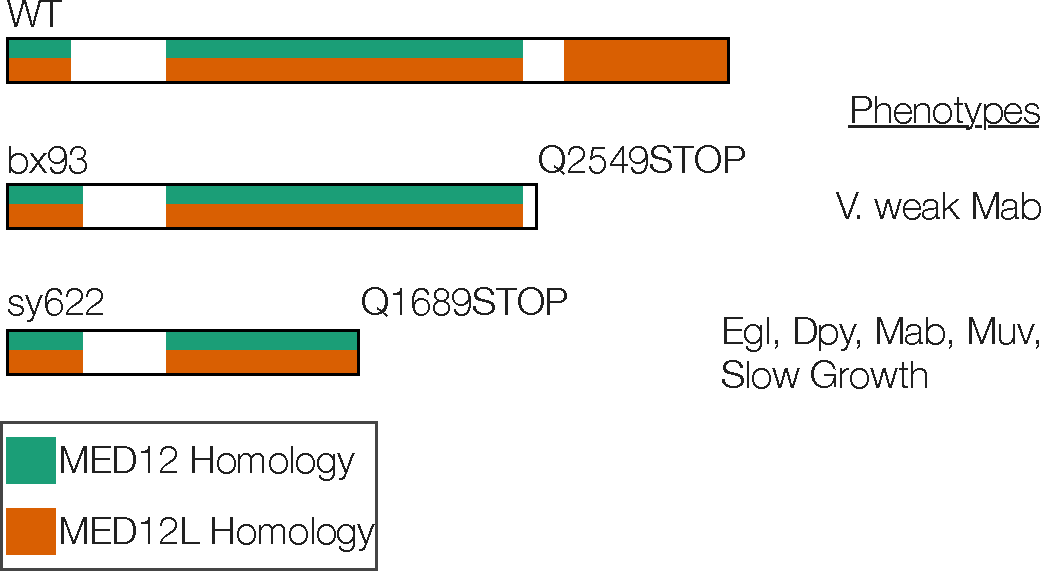
\includegraphics[width=0.3\textwidth]{../figs/gene_model_dpy22.pdf}
  \caption{
    The \dpy{} allelic series, consisting of two amino acid truncations. Diagram
    of the \protein{mdt-12} wild-type protein and the protein product of
    \emph{bx93} and \emph{sy622} alleles.
    % Conservation between \protein{mdt-12} and a human ortholog is shown in color.
    }
\label{fig:dpy22}
\end{figure}

Expression profiles have the potential to facilitate dissection of molecular
structures within genes. For the \dpy{} allelic series, we found that the
perturbations caused by the weak loss-of-function allele, \emph{bx93}, are
entirely contained within the perturbations caused by the strong
loss-of-function allele, \emph{sy622}. Further, we found three phenotypic
classes affected by \dpy{}. For one class, termed the \emph{sy622}-specific
class, the \emph{bx93} homozygote, but not the \emph{sy622} homozygote, shows
wild-type functionality. In a \emph{trans}-heterozygote of \emph{sy622/bx93}
these perturbations are suppressed to wild-type levels from the \emph{sy622}
levels, which shows that \emph{bx93} is wild-type dominant for this phenotype. A
second class, called the \emph{sy622}-associated class, similarly shows
wild-type functionality in the \emph{bx93} homozygote but not in the
\emph{sy622} homozygote, yet in the \emph{trans}-heterozygote these
perturbations are modulated in a gene-dosage dependent manner. Finally, we
identified a third class, called the \emph{bx93}-specific class, which contained
genes that were altered in both homozygotes, but which showed an expression
level most similar to the \emph{bx93} homozygote, showing that \emph{bx93} has a
dominant mutant phenotype for this subset. For each class, we were able to
quantitatively measure the dominance level of each allele.


\section*{Results}
\subsection*{A conceptual framework for analyzing allelic series}
Allelic series offer a way to study the functional units within a gene without
requiring prior knowledge about the molecular structure of the mutations
involved. Alleles are placed in \emph{trans} to each other to check whether one
allele is dominant or co-dominant over the other for a given phenotype. These
dominance relationships can then be used to identify functional units within a
gene. To perform an allelic series analysis using transcriptome profiling, we
needed to identify transcriptional modules that corresponded to different
phenotypes, and, subsequently, test the alleles for dominance or semidominance
at these modules. We reasoned that these modules would represent phenotypic
classes that directly correspond to potentially observable phenotypes associated
with any two alleles for a given gene.

For arbitrary alleles, it is possible to imagine that two alleles impact exactly
the same set of phenotypes; impact entirely disjoint phenotypes; or share
some phenotypes but not others. It is also possible to imagine that the alleles
share dominance relationships that may or may not be the same for each genotype.
The results for any allelic series can be hypothesized and represented as a
Venn diagram (see Fig.~\ref{fig:framework}), where the circles represent
transcripts that are differentially expressed in one genotype relative to the
wild type control, and overlaps between circles represent the fact that a set of
transcripts is differentially expressed in the overlapping genotypes relative to
the wild type. Crucially, different genetic scenarios may be expected to
generate a specific number of phenotypic classes.

Although the diagrams can be drawn for each genetic scenario, differential
expression analyses always have a number of false positive and false negative
hits. After idealizing a number of genetic scenarios, we asked what the effect
of statistical noise would be on the number of classes. In every case,
statistical artifacts lead to the creation of more phenotypic classes than would
be expected. In some cases, the statistically artifactual classes can outnumber
the real number of classes by a factor of 6. Since each class can be interpreted
in terms of functional units, failure to identify artifactual classes could
contribute disproportionally to the inferred complexity of the gene under study.
For example, if two alleles were genetically identical, statistical artifacts
would still be expected to generate 6 artifactual classes, each containing a
few genes, if the two homozygotes and the \emph{trans}-heterozygote were
sequenced simultaneously. Instead of concluding that the alleles are genetically
identical, we might conclude that the alleles have a shared core activity, but
that they differ in their specific activities for small, yet highly specific,
set of genes. This pitfall highlights the importance of signal-to-noise analyses
that can accurately identify classes that have high noise. These analyses should
also ideally be able to distinguish the contribution of false positive hits,
which tend to create classes that must be ignored entirely, from false negative
hits, which tend to create classes that could safely be re-classified into
the correct categories.

We developed a conceptual method, which we call false hit analysis, that is
in theory capable of identifying classes with low signal-to-noise ratios and
that can identify whether the noise contribution is mainly from false positive
or false negative hits. Briefly, to perform a false hit analysis, an idealized
Venn diagram must be derived. The problem of selecting an appropriate Venn
diagram is not solved generally. After selecting a hypothesized Venn diagram,
the sizes of each class are estimated from the data. These sizes can then be
used to re-calculate the sizes of classes due to the estimated false positive
and false negative rates. If the size of a class from the false hits is
similar to the size of the equivalent observed class, then this class should be
considered artifactual.


\begin{figure*}
  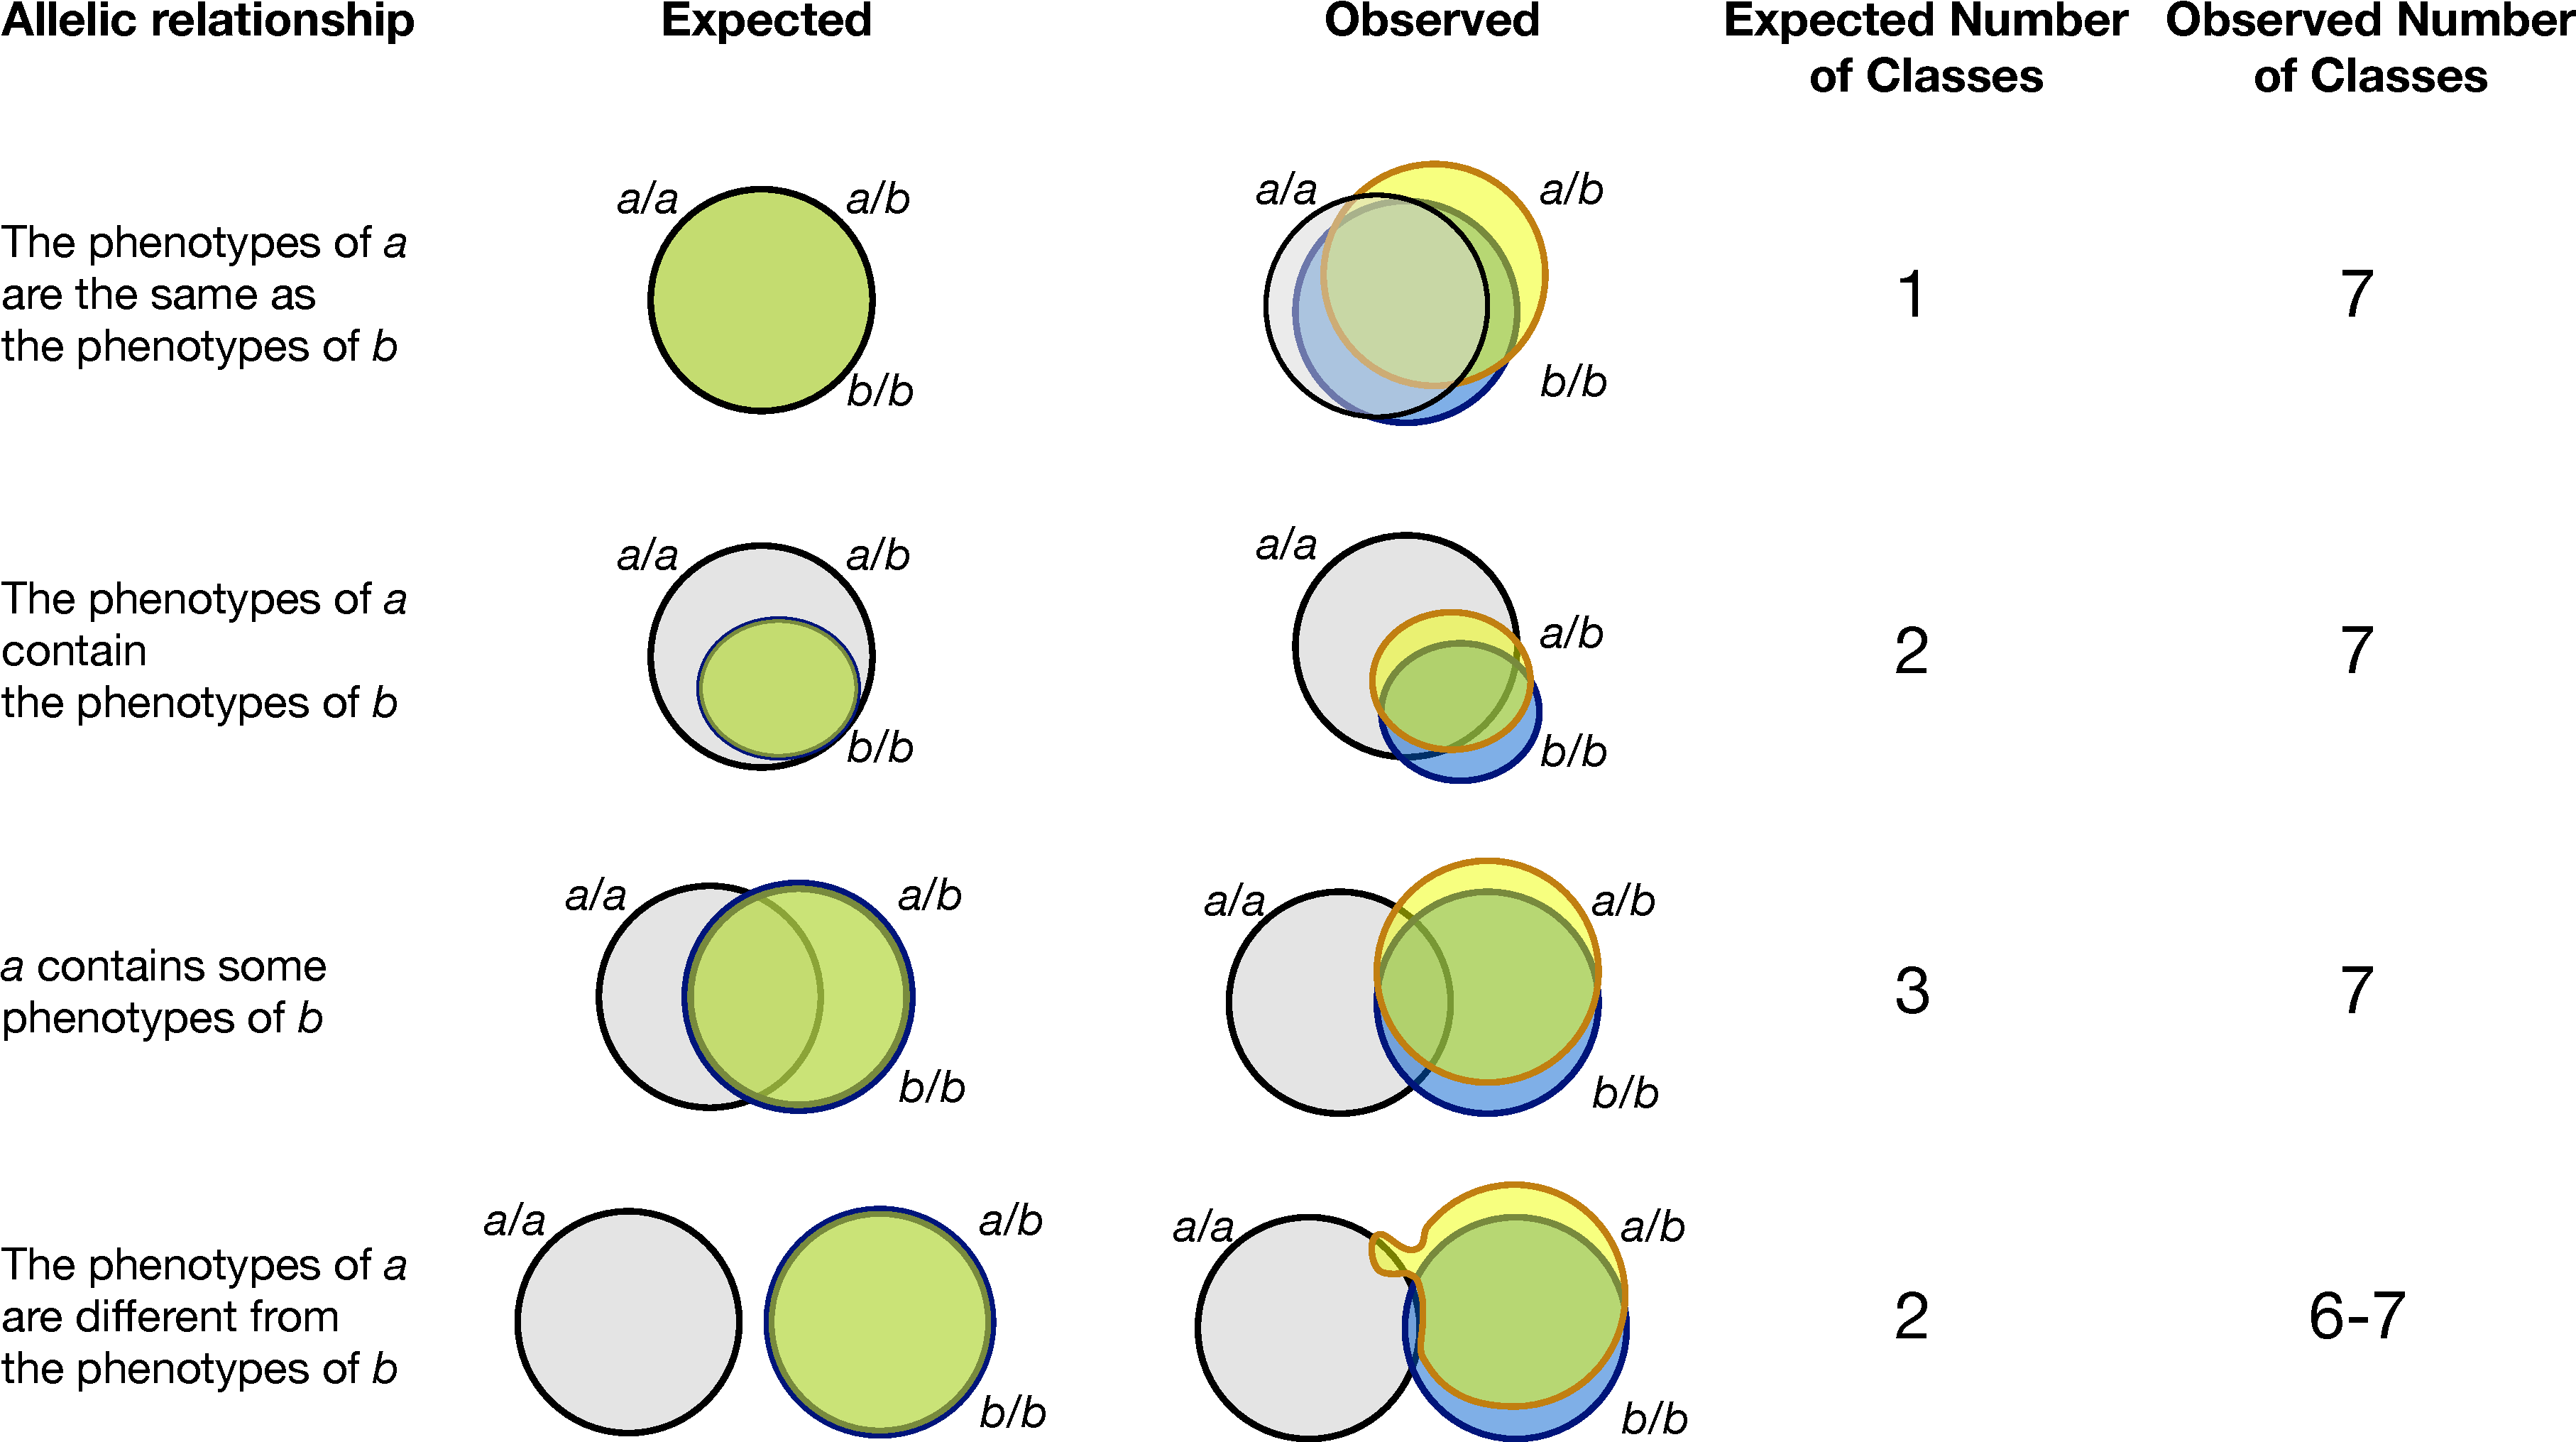
\includegraphics[width=\textwidth]{../figs/AllelicAnalysis_With_Het}
  \caption{
  The expected Venn diagrams for two alleles, \emph{a} and
  \emph{b}, if the two homozygotes and a \emph{trans}-heterozygote are
  sequenced for various possible scenarios. The circles represent the transcripts
  that are differentially expressed in a given genotype relative to a wild type
  control. In all scenarios, we assume the
  \emph{a} allele is recessive to \emph{b}, and we do not consider the
  possibility of gene dosage for simplicity. In theory, different scenarios
  should have a different number of phenotypic classes, but statistical artifacts
  (false positive and negative hits) always inflate the observed number of
  classes.
  }
\label{fig:framework}
\end{figure*}


\subsection*{Strong and weak loss-of-function alleles of \gene{mdt-12} show
             different transcriptomic profiles}
We sequenced in triplicate cDNA synthesized from mRNA extracted from
\emph{sy622} homozygotes, \emph{bx93} homozygotes,
\emph{trans}-heterozygotes of both alleles and wild-type controls at a depth of
20 million reads per replicate. This allowed us to quantify expression levels of
21,954 protein-coding isoforms. We calculated differential expression with
respect to a wild-type control using a general linear model
(see~\nameref{sec:methods}). Differential expression with respect to the
wild-type control for each transcript $i$ in a genotype $g$ is measured via a
coefficient $\beta_{g, i}$, which can be loosely interpreted as the natural
logarithm of the fold-change. Positive $\beta$ coefficients indicate
up-regulation with respect to the wild-type, whereas negative coefficients
indicate down-regulation. Transcripts were tested for differential expression
using a Wald test, and the resulting $p$-values were transformed into $q$-values
that are correcteed for multiple hypothesis testing. Transcripts were considered
to have differential expression between wild-type and a mutant if the associated
$q$-value of the $\beta$ coefficient was less than 0.1. At this threshold, 10\%
of all differentially expressed genes are expected to be false positive hits.

Using these definitions, we found \weakn{} differentially expressed
genes in the  \emph{bx93} homozygote transcriptome, and \strongn{}
differentially expressed genes in the \emph{sy622} homozygote transcriptome
(see Fig.~\ref{fig:false_hit}).

\subsection*{Transcriptome profiling of \gene{mdt-12}
             \emph{trans}-heterozygotes}
We also sequenced \emph{trans}-heterozygotic animals with genotype
\gene{dpy-6(e14) bx93/+ sy622}. This \emph{trans}-heterozygote appears
phenotypically wild-type, resembling the \emph{bx93} mutant
morphologically~\cite{Moghal2003}. The \emph{trans}-heterozygote transcriptome
had \transn{} differentially expressed genes.

\subsection*{False hit analysis identifies four phenotypic classes}
Overlapping three sets of differentially expressed genes from different
genotypes can generate at most seven categories. Each of these seven categories
could be interpreted biologically if the population is believed to arise from
real effects. If these populations are small, however, there is a real chance
that they represent statistical noise, and are not biologically meaningful.
If that is the case, these populations may consist largely of genes that are
mis-classified and belong to a different cluster, in which case they should be
re-classified into the most likely cluster, if it can be determined.

We identified three categories of genes that were most likely to be influenced
by statistical noise due to their small size. These populations were those that
encompassed genes differentially expressed in  \emph{bx93} homozygotes and one
other genotype, as well as genes that were differentially expressed specifically
in \emph{bx93} homozygotes.

These three categories stand out as candidates for statistical noise not just
because of their small size, but also because of the extraordinary biological
interpretations required to make sense of them. For example, if there truly is
a population of genes that is only perturbed in homozygotes of either allele but
not in the \emph{trans}-heterozygote, then this means that the two alleles are
somehow intragenically complementing to produce wild-type function. Given the
molecular nature of the mutations, this interpretation is unlikely to be correct.

To perform a false hit analysis, we imagined an idealized scenario where the
perturbations in \emph{bx93} homozygotes were present in all thre genotypes. We
also imagined that in this scenario the \emph{trans}-heterozygote did not exhibit
any perturbations not present the \emph{sy622} homozygote. In this simplified
scenario, we could model where false positive and false negative hits were most
likely to fall (see Fig.~\ref{fig:false_hit}). Next, we present the results of
our hit analysis for each perturbation category.

\begin{figure}
  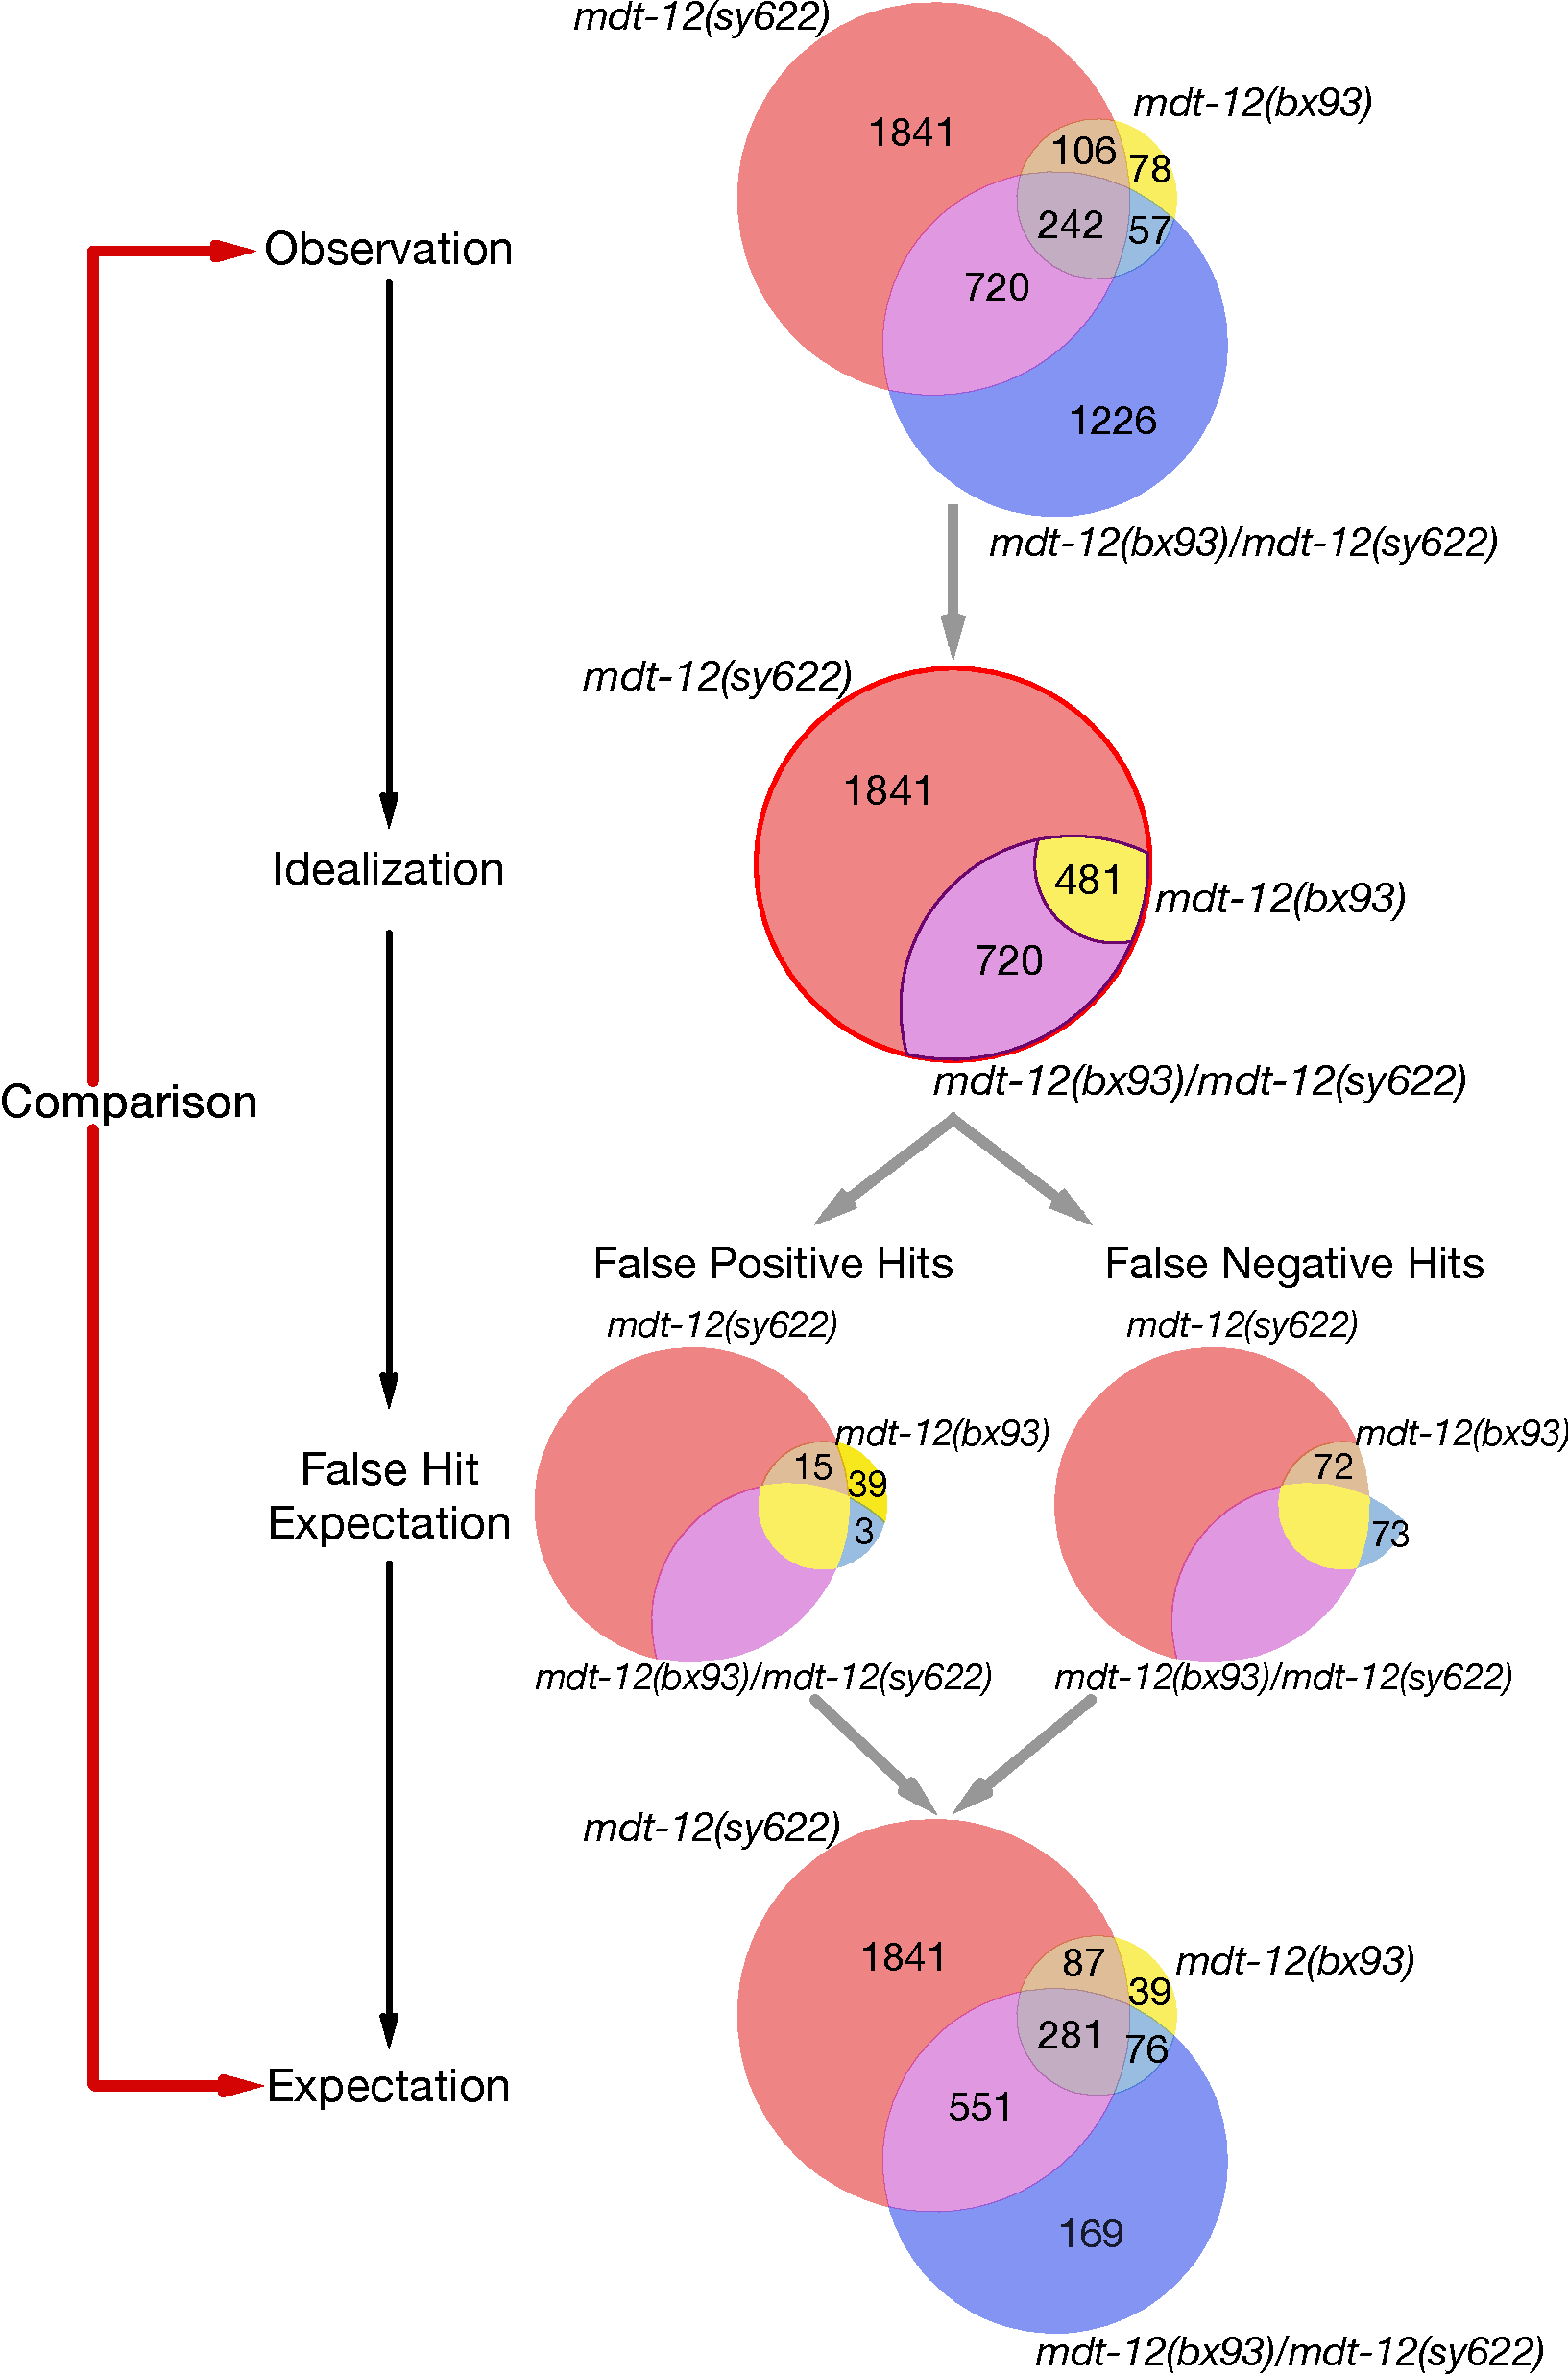
\includegraphics[width=0.5\textwidth]{../figs/false_hit_analysis.pdf}
  \caption{False hit analysis. To assess the extent to which statistical
  artifacts could affect the interpretation of certain intersections, we
  first idealized the Venn diagram and asked whether false positive and
  false negative results could distort the diagram back to its original
  shape. We estimated the false negative rate at 15\% and used a false positive
  rate of 10\%. For simplicity, only false hit analysis for \emph{bx93} groups
  is shown. False hits can explain the existence of a groups of genes that
  are differentially expressed in \emph{bx93} homozygotes only, in \emph{bx93}
  homozygotes and \emph{trans}-heterozygotes, and in \emph{bx93} homozygotes
  and \emph{sy622} homozygotes. Genes that are solely expressed in \emph{bx93}
  homozygotes are unlikely to exist, whereas genes that are differentially
  expressed in \emph{bx93} homozygotes and one other genotype are probably
  mis-classified and should be differentially expressed in all genotypes. The
  \emph{trans}-heterozygote specific class cannot be explained by statistical
  artifacts.
  }
\label{fig:false_hit}
\end{figure}

We identified 78 genes that are differentially expressed exclusively in
\emph{bx93} homozygotes. At a false positive rate of 10\% (our defined cut-off)
we expect 48 genes to be falsely called as differentially expressed in
\emph{bx93} homozygotes. The probability that such a false positive is also
differentially expressed in another genotype is 20\% (4,392 transcripts
identified between the two other genotypes divided by 21,954 the total number of
transcripts that were successfully sequenced). Thus, on average we expect 39
false positive hits to be classified into the \emph{bx93}-specific class. On
average, half of all genes in the \emph{bx93}-specific class would be expected
to be the result of statistical artifacts. Statistical noise is therefore a
major contributor towards the existence of this class. Since the biological
interpretation of this class is unclear and requiring extraordinary evidence, we
find the most parsimonious explanation to be that the \emph{bx93}-specific class
does not exist.

We estimated that statistical noise could account for $>80$\% of the genes that
were differentially expressed in both \emph{bx93} and \emph{sy622} homozygotes
and not differentially expressed in the \emph{trans}-heterozygote. Further, we
estimated that statistical artifacts could explain $>80$\% of the transcripts
that were differentially expressed in the \emph{trans}-heterozygote and
\emph{bx93} homozygotes but not in \emph{sy622} homozygotes. For both of these
populations, we estimate that the majority of the false hits emerge from false
negative results. In other words, most of the noise in these populations is the
result of mis-classification. Finally, the biological interpretation of either
population is implausible given the molecular nature of the alleles. Taken
together, a false hit analysis of these two categories strongly suggests that
they contain genes that have been mis-classified and which most likely are
differentially expressed in all three genotypes.

A false hit analysis identified four non-overlapping phenotypic classes (see
Fig.~\ref{fig:venn}). We use the term allele- or genotype-specific to refer to
groups of transcripts that are solely perturbed in a single genotype. On the
other hand, we use the term allele-associated to refer to those groups of
transcripts that are perturbed in at least two genotypes. We identified a
\emph{sy622}-associated phenotypic class, which consisted of 720 genes
differentially expressed in \emph{sy622} homozygotes and in
\emph{trans}-heterozygotes, but which were not differentially expressed in
\emph{bx93} homozygotes. We also identified a \emph{bx93}-associated phenotypic
class. Following the argument of the previous paragraph, this class included all
genes that were differentially expressed in \emph{bx93} homozygotes and at least
one other genotype, since it is likely that of these genes should actually be
differentially expressed in all genotypes. As a result, this class contains 403
genes. We also identified a \emph{sy622}-specific phenotypic class (1,841 genes)
and a \emph{trans}-heterozygote-specific phenotypic class (1,226 genes). Having
identified these phenotypic classes, we set out to confirm whether each class
actually behaved as an independent phenotypic module in an allelic series and
whether each class could be interpreted biologically to shed light on the
functions of \dpy{}.


\begin{figure}
  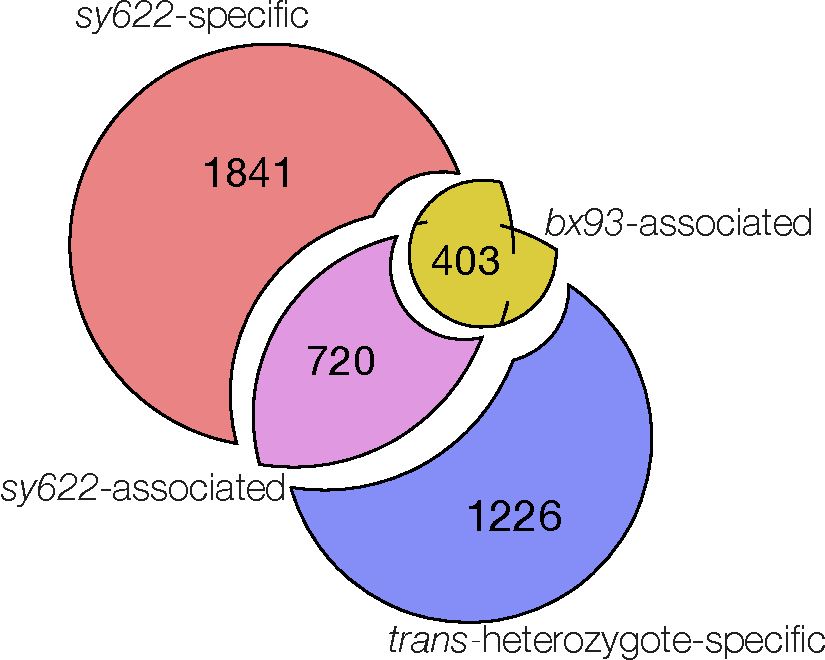
\includegraphics[width=0.5\textwidth]{../figs/exploded_venn.pdf}
  \caption{
  Transcripts under the control of \dpy{} belong to distinct phenotypic
  classes. Exploded Venn diagram highlighting the four identified phenotypic
  classes.
  }
\label{fig:venn}
\end{figure}

\subsection*{Different phenotypic classes behave differently in an
            \emph{sy622} homozygote}
We asked whether these classes had perturbation distributions distinct from each
other within a single homozygote. Specifically, we wanted to test whether these
sets behaved as randomly selected sets. If this were the case, then within a
single genotype, each class would be expected to have the same distribution of
perturbations (see Fig.~\ref{fig:classes}). We found that that the $\beta$
coefficients of isoforms within the \emph{bx93}-associated phenotype on average
had the largest absolute value (mean: $1.2$). The \emph{sy622}-associated
phenotype had a smaller range of perturbations compared to the
\emph{bx93}-associated phenotype (95th percentiles of the two distributions: 2.9
versus 3.2, respectively), and a statistically smaller median (0.91 vs 1.2,
respectively, $p < 10^{-6}$, non-parametric boostrap). The medians of the
\emph{sy622}-specific and -associated classes were the same ($p=0.15$). There
are systematic differences between the behaviors of each class. This rejects the
null hypothesis that the transcripts in each class were randomly selected.

% to make figure span two columns in twocolumn mode, use figure*
\begin{figure*}
  \centering{}
  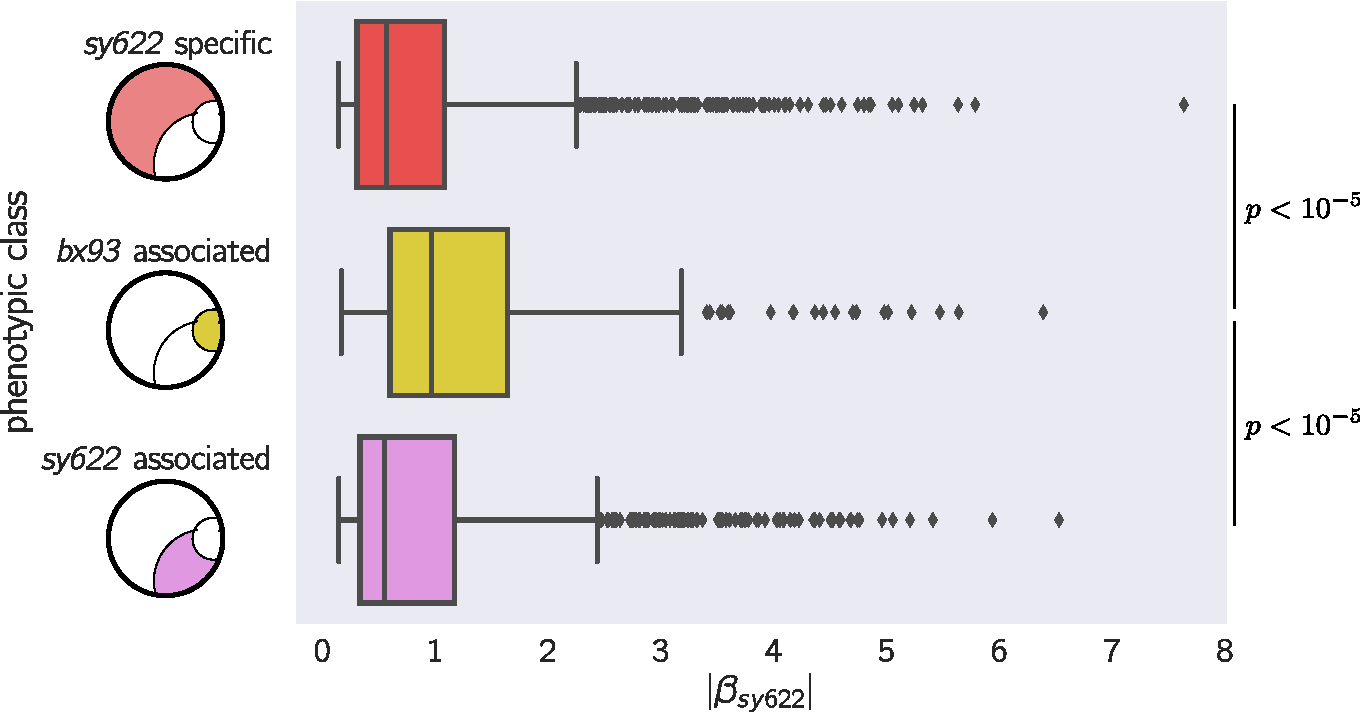
\includegraphics[width=0.75\textwidth]{../figs/dpy22_classes.pdf}
  \caption{
    Within the \emph{sy622} homozygote mutant, transcripts whose differential
    expression pattern places them in different phenotypic classes have
    statistically different distributions. The lines within the boxes show the
    25\textsuperscript{th}, 50\textsuperscript{th}, and 75\textsuperscript{th}
    percentiles. Whiskers show the 0\textsuperscript{th} and
    100\textsuperscript{th} percentiles, with the exception of outliers
    (diamonds). Diagrams show what genotypes each gene class is expressed in,
    but the magnitude of the perturbation plotted always corresponds to the
    \emph{sy622} mutant. The x-axis shows the absolute magnitude of the
    perturbation for each transcript in \emph{sy622} homozygotes,
    $|\beta_{sy622}|$. The medians of the \emph{sy622}-specific and the
    \emph{sy622}-associated classes were statistically significantly different
    from the median of the \emph{bx93}-specific class, as assessed by a
    non-parametric bootstrap test.
  }
\label{fig:classes}
\end{figure*}

\subsection*{Dominance can be quantified in transcriptomic phenotypes}
Dominance relationships between alleles are phenotype-specific. In other words,
an allele can be dominant over another for one phenotype, yet not for others. An
example is the \gene{let-23} allelic series---nulls of \gene{let-23} are
recessive lethal (Let) and presumably also recessive vulvaless (Vul) relative to
the wild-type allele. The \emph{sy1} allele of \gene{let-23} is dominant viable
relative to null alleles, but is recessive Vul~\cite{Aroian1991} to the
wild-type allele. Above, we postulated that there are four phenotypic classes,
three of which are composed of genes whose expression is significantly perturbed
in the \emph{sy622} homozygote. If these classes are indeed modular phenotypes,
then the dominance relationships within each class should be the same from gene
to gene. In other words, a single dominance coefficient should be sufficient to
explain the gene expression in the \emph{trans}-heterozygote for every gene
within a class.

To quantify this dominance, we implemented and maximized a Bayesian model (see
\nameref{sec:methods}). Briefly, we asked what the linear combination of $\beta$
coefficients from each homozygote would best predict the observed $\beta$ values
of the heterozygote, subject to the constraint that the coefficients added up to
1 (see \nameref{subsec:dominance}). We reasoned that if this was a modular
phenotype controlled by a single functional unit encoded within the gene of
interest, then a plot of the predicted $\beta$ values from the optimized model
against the observed $\beta$ values of the heterozygote for each transcript
should show the data falling along a line with slope equal to unity. Systematic
deviations from linear behavior would indicate that the transcripts plotted are
not part of a modular phenotypic class controlled by a functional unit.

\subsubsection*{The \emph{sy622}-specific class expression phenotype of the
                \emph{sy622} homozygote is complemented to wild-type levels by
                the presence of a \emph{bx93} allele}
Since our previous testing showed that the transcript expression of genes in
this class was dysregulated in \emph{sy622} homozygotes, and wild-type in both
\emph{bx93} homozygotes and \emph{trans}-heterozygotes we can conclude that
these transcripts are complemented to their wild-type levels by the presence of
the \emph{bx93} allele. Applying the Bayesian model yields identical results
($d_{bx93} = 1$). Thus, there is a module that has wild-type functionality in
the \emph{bx93} allele but is partially or completely deleted in the
\emph{sy622} allele. This functionality must require protein encoded between the
amino acid position 1,698 where the \emph{sy622} protein product truncates
prematurely, and the position 2,549 where the \emph{bx93} protein product ends.

\subsubsection*{The \emph{bx93} allele is dominant over the \emph{sy622} for the
                \emph{bx93}-associated phenotype}
We explored how expression levels of transcripts within the
\emph{bx93}-associated phenotypic class were controlled by these two alleles.
Transcripts in this class are differentially expressed in homozygotes of either
allele. Moreover, transcripts in this class are more perturbed in \emph{sy622}
homozygotes than in \emph{bx93} homozygotes. This is consistent with a single
functional unit that is impaired in the \emph{bx93} allele, and even more
impaired in the \emph{sy622} allele (see Fig.~\ref{fig:bx93_associated}).

If a single functional unit is being impaired, then we would expect these
alleles to form a quantitative allelic series for this phenotypic class. In a
quantitative series, alleles exhibit semidominance. We quantified the dominance
coefficient for this class and found that the \emph{bx93} allele is largely but
not completely dominant over the \emph{sy622} allele ($d_{bx93}=0.81$; see
Fig.~\ref{fig:bx93_associated}). Dominance in the context of an allelic series
indicates a qualitative allelic series, which is evidence that \protein{MDT-12}
protein produced from the \emph{bx93} allele has an intact functional unit that
is deleted in protein product from the \emph{sy622} allele. Mixed evidence for
quantitative and qualitative allelic series at this phenotypic class precludes a
definitive conclusion.

\begin{figure}
  \centering{}
  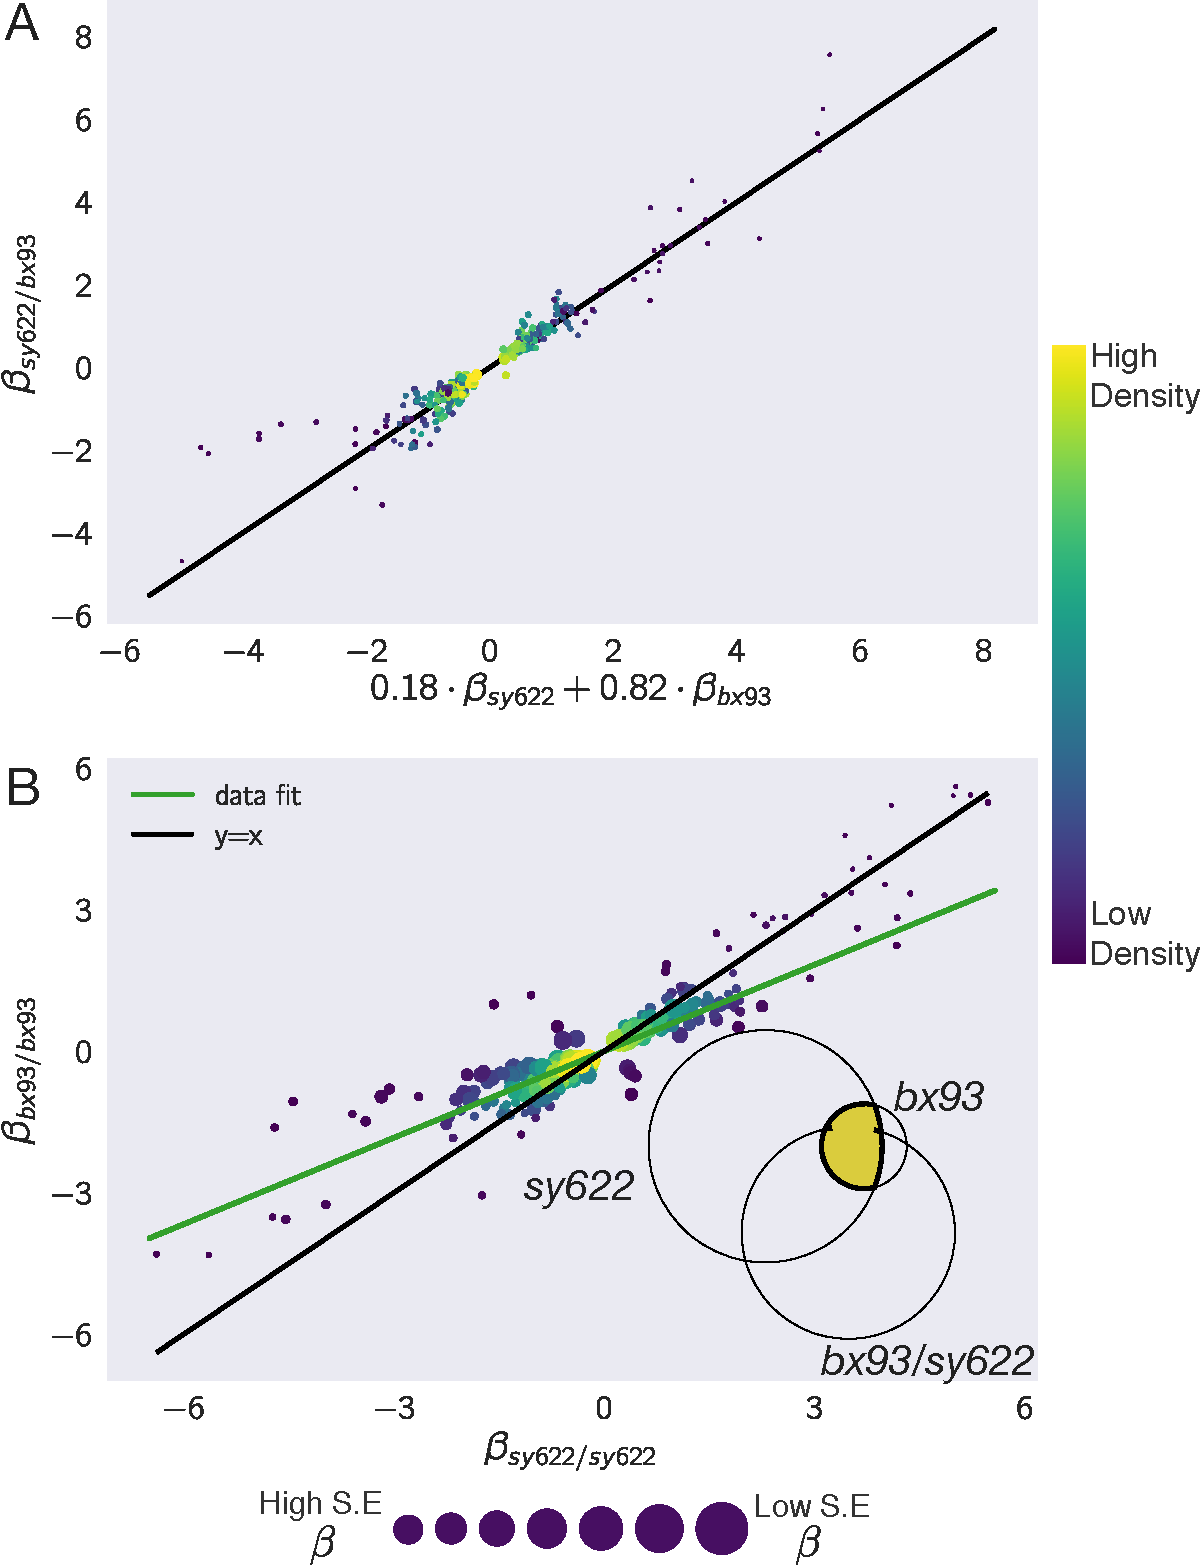
\includegraphics[width=0.5\textwidth]{../figs/bx93_associated_analysis.pdf}
  \caption{The \emph{bx93}-associated class has properties of both quantitative
    and qualitative allelic series.
    \textbf{A} In \emph{bx93}
    homozygotes, transcripts within the \emph{bx93}-associated class are
    less perturbed than in \emph{sy622}
    homozygotes. The line of best fit (green) is
    $\beta_{bx93/bx93}=0.56\cdot\beta_{sy622/sy622}$.
    \textbf{B} In a \emph{trans}-heterozygote, the \emph{bx93} allele is largely
    dominant over the \emph{sy622} allele for the expression levels of
    transcripts in the \emph{bx93}-associated class.
    In the graphs above, densely packed points are colored yellow as a visual
    aid. The size of the point is inversely proportional to the standard error
    of the $\beta$ coefficients.
    }
\label{fig:bx93_associated}
\end{figure}

\subsubsection*{The \emph{bx93} allele is semidominant with \emph{sy622} for the
                \emph{sy622}-associated phenotypic class}
We quantified the relative dominance of \emph{bx93} and \emph{sy622} on the
expression level of transcripts that belonged to the \emph{sy622}-associated
class. We found that both alleles are semidominant ($d_{bx93} = 0.51$). This
suggests that there is a structure distributed evenly throughout the gene
body starting the first amino acid position and ending before position 2,549.
Since the two alleles are semidominant for transcript expression in this class,
the functionality encoded in this gene must be dosage-dependent for this model
to hold.

\subsection*{The \emph{sy622}-specific class is strongly enriched for a Dpy
             transcriptional signature}
\emph{bx93} homozygotic animals are almost wild-type, but careful measurements
show that they have a slight body length defect causing them to be slightly Dpy,
and \emph{sy622} homozygotic animals are known to be severely
Dpy~\cite{Moghal2003}, but this phenotype is complemented almost to \emph{bx93}
levels when this allele is placed in \emph{trans} to the \emph{sy622} allele.
The only class that is fully complemented to wild-type levels is the
\emph{sy622}-specific class. Therefore, we hypothesized that the
\emph{sy622}-specific class should show a strong transcriptional Dpy signature.

To test this hypothesis, we derived a Dpy signature from two Dpy mutants
(\gene{dpy-7} and \gene{dpy-10}, DAA, CPR and PWS \emph{unpublished}) consisting
of 628 genes. We used this gene set to look for a transcriptional Dpy signature
in each phenotypic class using a hypergeometric probabilistic model
(see~\nameref{sec:methods}). We found that the \emph{sy622}-specific and
-associated classes were enriched in genes that are transcriptionally associated
with a Dpy phenotype. The \emph{bx93}-associated class also showed significant
enrichment (fold-change = 2.2, $p=4\cdot10^{-10}$, 68 genes observed). The
enrichment was of considerably greater magnitude in the \emph{sy622}-specific
class (fold-change enrichment = 3, $p=2\cdot 10^{-40}$, $167$ genes observed)
than the enrichment in the \emph{sy622}-associated class (fold-change = 1.9,
$p=9\cdot10^{-9}$, 82 genes observed) or in the \emph{bx93}-associated class.
Correlation analysis showed that a majority of the genes in the
\emph{sy622}-specific class were strongly correlated between the expression
levels in the Dpy signature and the expression levels in \emph{sy622}
homozygotes, while 25\% of the genes were anti-correlated (Spearman R = 0.42,
$p=6\cdot10^{-15}$, see Fig.~\ref{fig:dpy_phenotype}). If the anti-correlated
values are excluded from the Spearman regression, the statistical value of the
regression improves significantly (Spearman R = 0.94, $p=2\cdot10^{-108}$).
Taken together, this suggests that the \emph{sy622}-specific phenotypic class
contains a transcriptional signature that can be associated with the
morphological Dpy phenotype.

We also tested a hypoxia dataset~\cite{AngelesAlboresHIF}, since \emph{mdt-12}
is not known to be upstream of the \gene{hif-1}-dependent hypoxia response
in \cel{}. Enrichment tests revealed that the hypoxia response was significantly
enriched in the \emph{bx93}-associated (fold-change = 2.1, $p=10^{-8}$, 63 genes
observed), the \emph{sy622}-associated (fold-change = 1.9, $p=4\cdot10^{-8}$, 78
genes observed) and the \emph{sy622}-specific classes (fold-change = 2.4,
$p=9\cdot10^{-55}$, 186 genes observed). However, there was no correlation
between the expression levels of these genes in \dpy{} genotypes and the
expression levels expected from the hypoxia response. Although the hypoxia gene
battery can be found in \dpy{} mutants, these genes are not used to deploy a
hypoxia response, and the animals do not have a hypoxic-response phenotype.

\begin{figure}
  \centering{}
  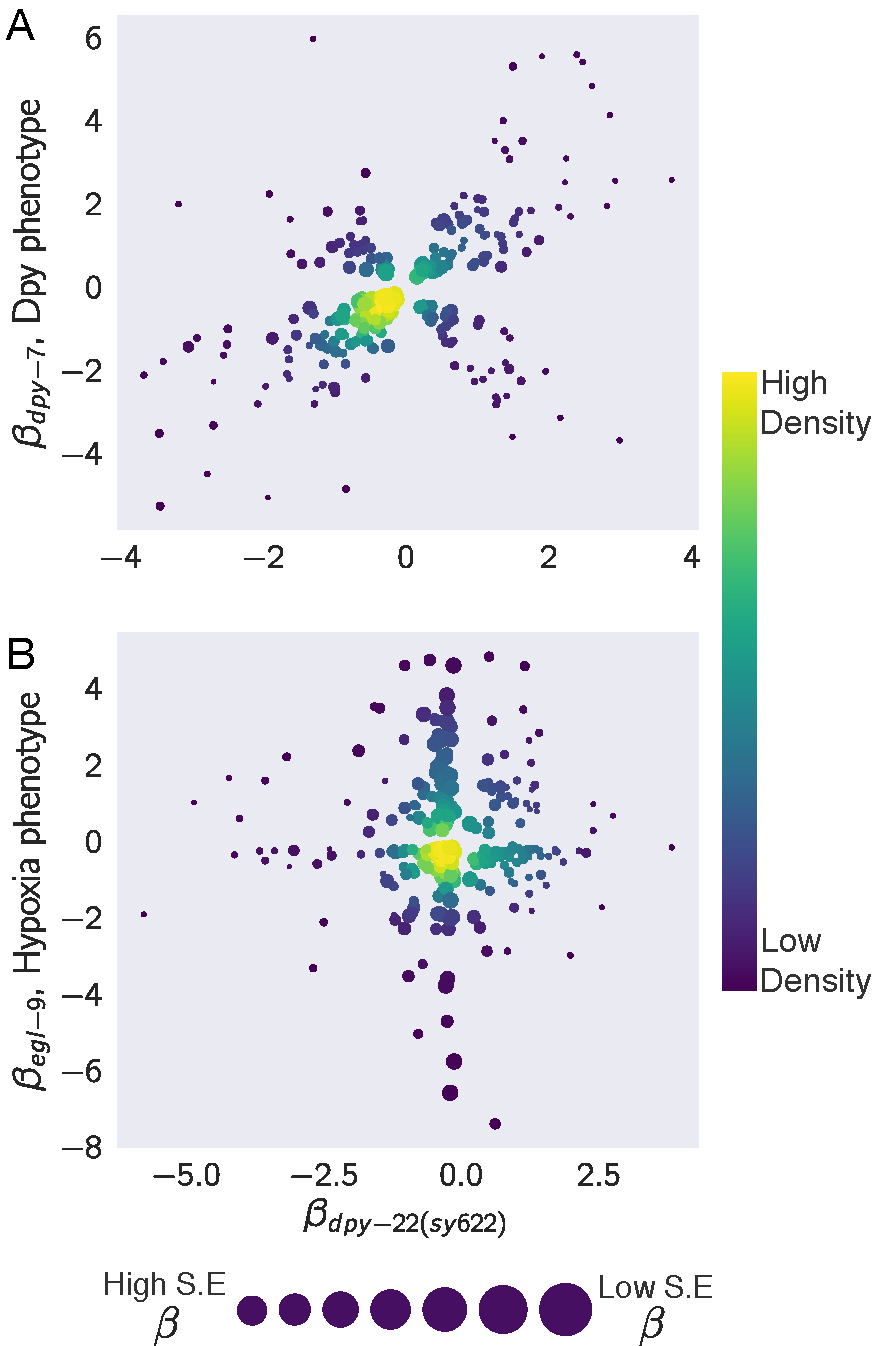
\includegraphics[width=0.5\textwidth]{../figs/dpy_phenotype.pdf}
  \caption{
    \emph{sy622} homozygotes show a transcriptional response associated with the
    Dpy phenotype. \textbf{A} We obtained a set of transcripts associated with
    the Dpy phenotype from \gene{dpy-7} and \gene{dpy-10} mutants. We identified
    the transcripts that were differentially expressed in \emph{sy622}
    homozygotes. Next, we plotted the $\beta$ values of each transcript in
    \emph{sy622} homozygotes against the $\beta$ values in a \emph{dpy-7}
    mutant. A significant portion of the genes are correlated between the two
    genotypes, showing that the signature is largely intact. 25\% of the genes
    are anti-correlated. \textbf{B} We performed the same analysis using a set
    of transcripts associated with the \gene{hif-1}-dependent hypoxia response
    as a negative control. Although \emph{sy622} is enriched for the transcripts
    that make up this response, there is no correlation between the $\beta$
    values in \emph{sy622} homozygotes and the  $\beta$ values in \emph{egl-9}
    homozygotes. In the plots, a colormap is used to represent the density of
    points. The standard error of the mean is inversely proportional to the
    standard error of $\beta_{mdt-12(sy622)}$.
    }
\label{fig:dpy_phenotype}
\end{figure}


\section*{Discussion}
\label{sec:conclusions}
\subsection*{Allelic series using transcriptomic phenotypes can dissect the
             functional units of a gene}
We have shown that whole-organism transcriptomic phenotypes can be analyzed in
the context of an allelic series to partition the transcriptomic effects of a
large, pleiotropic gene into separable classes. Analysis of these modules can
inform structure/function predictions at the molecular level, and enrichment
analysis of each class can be subsequently correlated with other morphologic or
behavioral phenotypes. This method shows promise for analysing pathways that
have major effects on gene expression in an organism, and which do not have
complex, antagonistic tissue-specific effects on expression. Given the
importance of allelic series for fully characterizing genetic pathways, we are
optimistic that this method will be a useful addition towards making full use of
the potential of these molecular phenotypes. Specifically, allelic series
coupled with false hit analyses show great promise to identify distinct
phenotypic classes that would be difficult or impossible to measure using
standard methods. The sensitivity and quantitative nature of transcriptomic
phenotypes makes identification of these phenotypes considerably more feasible.
Once the phenotypic classes have been identified, dominance and enrichment
analyses can be performed easily with significant statistical power. These
properties highlight the power of coupling the genetical properties of \cel{}
with next-generation sequencing methods.

\subsection*{A structure/function diagram of \dpy{}}
Our results strongly suggest the existence of various functional units in \dpy{}
that control distinct phenotypic classes (see Fig.~\ref{fig:domains}). The
\emph{sy622}-specific class of transcripts is regulated normally in the presence
of the \emph{bx93} allele, indicating that the mutated protein product retains
wild-type functionality for regulating these genes. This functionality is
decreased or absent in \protein{mdt-12} produced from the \emph{sy622} allele.
Therefore, the functional unit that controls this class, functional unit 1 (FC1),
must require sequence between amino-acid position 1,689 and position 2,549.

A similar argument can be made for a functional unit that controls
\emph{sy622}-associated transcripts, functional unit 2 (FC2). These genes are
strongly perturbed in \emph{sy622} homozygotes and they are also perturbed in
\emph{bx93/sy622} \emph{trans}-heterozygotes, albeit to a lesser degree. For
this argument to hold, however, the functional unit must work in a
dosage-dependent manner, since the \emph{bx93} allele is semidominant with the
\emph{sy622} allele, and this unit is likely intact in the protein product made
by the \emph{bx93} allele. This is in contrast to FC1, which is not
dosage-dependent.

Evidence in favor of a \emph{bx93}-associated functional unit was mixed.
Although dominance analysis suggested that the \emph{bx93} allele was largely
dominant over the \emph{sy622} allele for expression levels of genes in this
class, the expression of these genes deviated from wild-type levels in both
alleles. The latter suggests that the \emph{bx93}-associated module is perturbed
quantitatively in both alleles, whereas dominance analyses favor an
interpretation where the module is present in one allele but not in the other.
One possibility is that the \emph{bx93}-associated function we observed is the
joint activity of two distinct effectors, functional units 3 and 4 (FC3, FC4,
see Fig.~\ref{fig:domains}). In this model, FC4 loses partial function in the
\emph{bx93} allele, whereas the FC3 retains its complete activity. This leads to
non-wild-type expression levels of the \emph{bx93}-associated class of
transcripts. In the \emph{sy622} allele, FC4 is further impaired, causing an
increase in the severity of the observable phenotype. A rigorous examination of
this model requires studying alleles that mutate the region between Q1689 and
Q2549 using homozygotes and \emph{trans}-heterozygotes. Future work should be
able to establish how many modules exist in total, and how they may
interact to drive gene expression. The phenotypic classes identified here could
be compared against transcriptomic signatures from other transcription factors
to identify candidate cofactors.

\begin{figure}
  \centering{}
  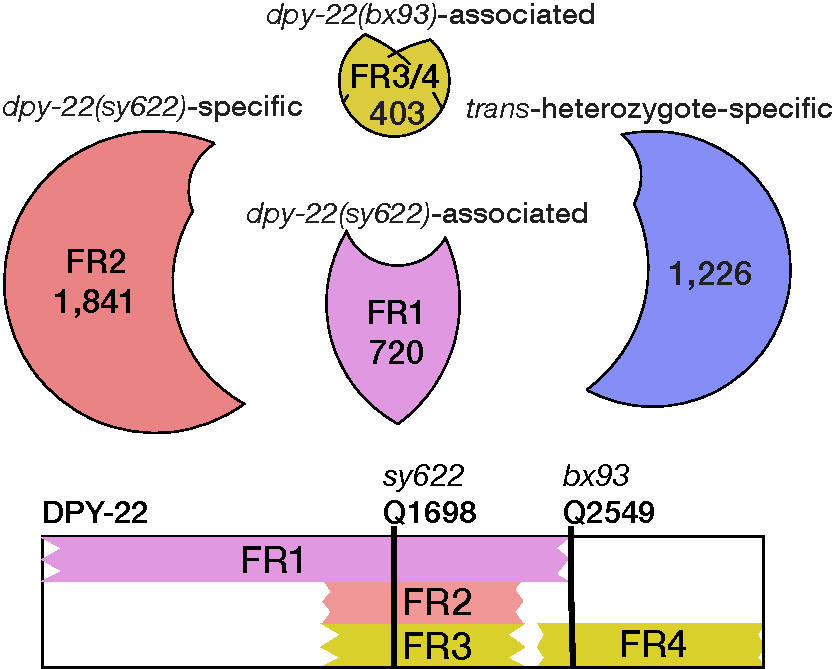
\includegraphics[width=0.5\textwidth]{../figs/inferred_domains.pdf}
  \caption{
    The functional units associated with each phenotypic class can be
    mapped to intragenic locations. The beginning and end positions of
    these functional units are unknown,
    so edges are drawn as ragged lines. Thick horizontal lines show the
    limit where each function could end, if known. We postulate that the
    \emph{bx93}-associated class is controlled by two functional units, FC3 and
    FC4, in the tail region of this gene. Some of the modules shown may
    represent the same structures. Future experiments are required to make a more
    complete determination of the number and nature of these modules.
  }
\label{fig:domains}
\end{figure}


\subsection*{Controlling statistical artifacts}
Transcriptomic phenotypes generate large amounts of information that can be used
to determine functional units. However, due to the large number of tests
performed, false positive and false negative events occur frequently enough to
create populations of transcripts that have anomalous behaviors. It is necessary
to identify what modules or populations are most at risk of these events and to
what extent these modules may be polluted by false signals to prevent
over-interpretation. In our experiment, we can estimate statistical noise in
each population. There is a rich literature in genomics devoted to controlling
and estimating false positive rates~\cite{Storey2003,Benjamini1995}, but false
negative rates have largely been ignored because they do not create spurious
signal in simple experimental designs and because there is ample signal in most
RNA-seq experiments. For allelic series experiments to be successful, systematic
algorithms to estimate and control false negative rates, and to identify the
populations most at risk for enrichment of false hits, must be developed,
because false negative hits can create populations of genes that have
fantastical biological behaviors (such as contrived examples of intragenic
complementation or dosage models).

We performed a false hit analysis, estimating the false negative rate at 15\%,
to identify the clusters or classes of genes most at risk for statistical noise.
As a general rule, small clusters or classes should be viewed with skepticism,
particularly if the biological interpretation is complex. To perform a
false hit analysis, we found it crucial is to appropriately idealize the shape
of the Venn diagram. This idealized Venn diagram can then be ``squeezed'' with
false negative and false positive rates to observe how it deforms. The deformed
diagram can then be compared with reality to estimate the contribution of false
hits to the existence of each class.

\subsection*{The \emph{trans}-heterozygote specific phenotypic class is not a
             statistical artifact}
In our study, we found a class of transcripts that were exclusively
differentially expressed in \emph{trans}-heterozygotes. The size of this class,
1226 genes, means it cannot be a statistical artifact. As a result, this class
must be interpreted either as a legitimate aspect of \dpy{} biology, possibly
reflecting dosage- or tissue-specific effects, or as a strain-specific artifact.
The genotype of the heterozygote includes a mutation at the \gene{dpy-6} locus
which acts as a cis-marker for the \emph{bx93} mutation. One possibility is that
the \emph{dpy-6} loss-of-function mutation is not recessive for transcriptomic
phenotypes and is responsible for the dysregulation of the new genes observed in
the heterozygote. Another possibility is that the \emph{dpy-6} strain had
background mutations that affect gene expression levels in a complex manner.
These issues could be addressed by re-generating the alleles used in this study
using genome engineering tools like CRISPR Cas9, which have few off-target
effects in \cel{}~\cite{Chiu2013}. However, even if these issues were addressed,
the biological interpretation of this class is not straightforward.

Phenotypes that are exacerbated or are unique to \emph{trans}-heterozygotes
often indicate that the protein products of the two alleles are somehow
interfering with each other. This interference can often be the result of
physical interactions such as homodimerization, or through a dosage reduction of
a toxic product~\cite{Yook2005}. In the case of \dpy{} orthologs, the protein
products are not known to form oligomers. Instead, \protein{mdt-12} and its
orthologs are expected to assemble in a monomeric manner into the
\protein{cdk-8} Kinase Module.

A dosage model could explain the \emph{trans}-heterozygote specific class if the
dosage curve is bell-shaped. In this model, a switch is only activated at a very
specific \dpy{} gene dosage. Beyond this dosage, the switch remains off.
Although such a model explains the data, mechanisms that could generate such a
dosage curve are not immediately obvious. One possibility is that this switch is
enacted at the level of cell specification or cell division, and that at the
appropriate dosage of \dpy{}, two cells that would typically collaborate to form
a phenotype now act antagonistically, pushing \emph{trans}-heterozygotes into a
different state from the homozygotes. If this is the case, whole-organism
RNA-seq may have limited resolution to identify what tissues or cells are being
perturbed. Single-cell sequencing of \cel{} has recently been reported. As this
technique becomes more widely adopted, and with decreasing cost, single-cell
profiling of these genotypes may provide information that complements the
whole-organism expression phenotypes, perhaps explaining the mysterious origin
of this phenotype.

\subsection*{Analysis of allelic series using transcriptome-wide measurements}
% TODO: hughes, o'shea
The potential of transcriptomes to perform epistasis analyses has been amply
demonstrated~\cite{Dixit2016,Angeles-Albores2017}, but their potential to
perform allelic series analyses has been less studied. Though similar in some
respects, epistasis analyses and allelic series studies call for different
methods to solve different problems. To successfully perform an allelic series
analysis, we must be able to identify the number and identity of the phenotypic
classes, and a dominance analysis must be performed for each class to determine
whether the alleles interact qualitatively or quantitatively with each other.
Additionally, if an allelic series includes more than two alleles, the number of
experimental outcomes and the number of possible outcomes rapidly become large.

% TODO:Clustering citations
The general problem of partitioning a set of genes into phenotypic classes is a
common problem in bioinformatics. This problem has been tackled through
clustering, matrix-based methods such as PCA or non-negative
matrix factorization, or through q-value-based classification (as we have done
here). Although these methods can classify genes or transcripts into clusters,
by themselves they cannot ascertain the probability that any one cluster is real.
For allelic series studies, this represents a major problem, since each cluster
can in theory represent a new, independent functional unit within the molecular
structure of the gene under study. Failure to identify clusters that are the
result of statistical artifacts in general will cause researchers to identify
inflated numbers of functional units within a molecular structure that appear to
behave in a biologically spectacular fashion. We attempted to solve this problem
for our series by estimating contributions of statistical noise to each class,
although a challenge is that we do not know the false negative rate in our
experiment. For our analysis, we exploited the molecular structure of our
alleles (nested truncations) to create an idealized version of how gene clusters
should behave. We then used our false positive rate and an estimated false
negative rate to estimate the signal/noise ratio for each class. This method
allows us to identify false classes, and in so doing it also reduces the apparent
complexity of the molecular structure of the gene under study.

A challenge for allelic series studies will be the biological interpretation of
unexpected classes, such as the \emph{trans}-heterozygote specific class in our
analysis. This class is too large to be explained by statistical anomalies.
If this class is not an artifact of background or strain construction, the
biological interpretation of this class is still not clear. Moreover, even if
the biological interpretation of this class were clear, it is not immediately
apparent what experimental design could establish the veracity of our
interpretation. This problem could perhaps be ameliorated by correlating
transcriptomic signatures with more morphologic, behavioral or cellular
phenotypes, as has been done in single-cell studies~\cite{Lane2017}.

\subsection*{Expression profiling as a method for phenotypic profiling}
The possibility of identifying distinct phenotypes using expression profiling is
an exciting prospect. With the advent of facile genome editing technologies, the
allele generation has become routine. As a result, phenotypification is now the
rate-limiting step for genetic analyses. We believe that RNA-seq can be used in
conjunction with allelic series to exhaustively enumerate independent phenotypes
with minor effort. We should push to sequence allelic diversity to more fully
understand genotype-genotype variation.

\section*{Methods}
\label{sec:methods}
\subsection*{Strains used}
Strains used were N2 wild-type (Bristol),
PS4087 \gene{mdt-12(sy622)},
PS4187 \gene{mdt-12(bx93)},
%line break inserted below because \gene{...} doesn't linebreak well
and PS4176\\ \gene{dpy-6(e14) mdt-12(bx93)/ + mdt-12(sy622)}.
All lines were grown on standard nematode growth media (NGM) Petri plates seeded
with OP50 \ecol{} at 20\degree{}C~\cite{Brenner1974}.

\subsection*{Strain synchronization, harvesting and RNA sequencing}
All strains were synchronized by bleaching
P$_0$'s into virgin S. basal (no cholesterol or ethanol added) for 8--12 hours.
Arrested L1 larvae were placed in NGM plates seeded with OP50 at 20\degree{}C
and allowed to grow to the young adult stage (as assessed by vulval morphology
and lack of  embryos). RNA extraction was performed as described
in~\cite{AngelesAlboresHIF} and sequenced using a previously described
protocol~\cite{Angeles-Albores2017}.

\subsection*{Read pseudo-alignment and differential expression}
Reads were pseudo-aligned to the \cel{} genome (WBcel235) using
Kallisto~\cite{Bray2016}, using 200 bootstraps and with the sequence bias
(\texttt{--seqBias}) flag. The fragment size for all libraries was set to 200
and the standard deviation to 40. Quality control was performed on a subset of
the reads using FastQC, RNAseQC, BowTie and
MultiQC~\cite{Andrews2010,Deluca2012,Langmead2009,Ewels2016}. All libraries had
good quality scores.

Differential expression analysis was performed using
Sleuth~\cite{Pimentel2016a}. Briefly, we used a general linear model to identify
genes that were differentially expressed between wild-type and mutant libraries.
To increase our statistical power, we pooled wild-type replicates from other
published~\cite{} and unpublished analysis. All wild-type replicates were
collected at the same stage (young adult). In total, we had 10 wild-type
replicates from 4 different batches, which heightened our statistical power.
Batch effects were smaller than between-genotype effects, as assessed by
principal component analysis (PCA), except when switching between samples
constructed by different library methods. Wild-type samples constructed using
the same library method clustered together and away from all other mutant
samples. However, clustering wild-type samples by themselves revealed that the
samples clusters correlated with the person who collected them. Therefore, we
added batch correction terms to our model to account for batch effects from
library construction as well as from the person who collected the samples.

\subsection*{Non-parametric bootstrap}
We performed non-parametric bootstrap testing to identify whether two
distributions had the same mean. Briefly, the two datasets were mixed, and
samples were selected at random with replacement from the mixed population into
two new datasets. We calculated the difference in the means of these new
datasets. We iterated this process $10^6$ times. To calculate a $p$-value that
the null hypothesis is true, we identified the number of times a difference in
the means of the simulated populations was greater than or equal to the observed
difference in the means of the real population. We divided this result by $10^6$
to complete the calculation for a $p$-value. If an event where the difference in
the simulated means was greater than the observed difference in the means was
not observed, we reported the $p$-value as $p<10^{-6}$. Otherwise, we reported
the exact $p$-value. We chose to reject the null hypothesis that the means of
the two datasets are equal to each other if $p < 0.05$.

\subsection*{Dominance analysis}
\label{subsec:dominance}
We modeled allelic dominance as a weighted average of allelic activity. Briefly,
our model proposed that $\beta$ coefficients of the heterozygote,
$\beta_{a/b,i,\text{Pred}}$, could be modeled as a linear combination of the
coefficients of each homozygote:
\begin{equation}
  \beta_{a/b,i,\text{Pred}}(d_a) = d_a\cdot \beta_{a/a,i} +
                                   (1-d_a)\cdot \beta_{b/b,i},
\end{equation}
where $\beta_{k/k, i}$ refers to the $\beta$ value of the $i$th isoform in a
genotype $k/k$, and $d_a$ is the dominance coefficient for allele $a$.

To find the parameters $d_a$ that maximized the probability of observing the
data, we found the parameter, $d_a$, that maximized the equation:
\begin{equation}
    P(d_a|D,H,I) \propto \prod_{i \in S}
                   \exp{-\frac{{(\beta_{a/b,i,\text{Obs}} -
                                \beta_{a/b,i,\text{Pred}}(d_a))}^2}{
                                2\sigma_i^2}}
\end{equation}
where $\beta_{a/b,i,\text{Obs}}$ was the coefficient associated with the $i$th
isoform in the \emph{trans}-het $a/b$ and $\sigma_i$ was the standard error of
the $i$th isoform in the \emph{trans}-heterozygote samples as output by
Kallisto. $S$ is the set of isoforms that participate in the regression (see
main text). This equation describes a linear regression which was solved
numerically.

\subsection*{Code}
All code was written in Jupyter notebooks~\cite{Perez2007} using the Python
programming language. The Numpy, pandas and scipy libraries were used for
computation~\cite{VanDerWalt2011,McKinney2011,Oliphant2007} and the matplotlib
and seaborn libraries were used for data visualization~\cite{Hunter2007,Waskom}.
Enrichment analyses were performed using the WormBase Enrichment
Suite~\cite{Angeles-Albores2016}. For all enrichment analyses, a $q$-value of
less than $10^-3$ was considered statistically significant. For gene ontology
enrichment analysis, terms were considered statistically significant only if
they also showed an enrichment fold-change greater than 2.

\section*{Acknowledgements}
This work was supported by HHMI with whom PWS was an investigator, by the
Millard and Muriel Jacobs Genetics and Genomics Laboratory at California
Institute of Technology, and by the NIH grant U41 HG002223. This article
would not be possible without help from Dr.\ Igor Antoshechkin and Dr.\ Vijaya
Kumar who performed the library preparation and sequencing. We would like to
thank Carmie Puckett Robinson for access to the unpublished Dpy transcriptional
signature. Han Wang, Hillel Schwartz, Erich Schwarz and Porfirio Quintero
provided valuable input throughout the project.

%This is where your bibliography is generated.
\bibliography{citations}
\bibliographystyle{naturemag}

\end{document}
